%----------------------------------------------------------------------------------------
%    PACKAGES AND THEMES
%----------------------------------------------------------------------------------------

\documentclass[aspectratio=169,xcolor=dvipsnames]{beamer}
\usetheme{SimpleDarkBlue}

\usepackage{hyperref}
\usepackage{graphicx} % Allows including images
\usepackage{booktabs} % Allows the use of \toprule, \midrule and \bottomrule in tables
\usepackage[dvipsnames]{xcolor}
\usepackage{algorithm}
\usepackage[noend]{algpseudocode}
\usepackage[absolute,overlay]{textpos}
\usepackage{amssymb}

%----------------------------------------------------------------------------------------
%    TITLE PAGE
%----------------------------------------------------------------------------------------

\title{MCTS - Connect four}
\subtitle{Markov Decision Processes and Reinforcement Learning}

\author{Samuele Angheben}

\institute
{
    Trento University % Your institution for the title page
}
\date{\today} % Date, can be changed to a custom date

%----------------------------------------------------------------------------------------
%    PRESENTATION SLIDES
%----------------------------------------------------------------------------------------

\begin{document}

\begin{frame}
    % Print the title page as the first slide
    \titlepage
\end{frame}

\begin{frame}{Overview}
    % Throughout your presentation, if you choose to use \section{} and \subsection{} commands, these will automatically be printed on this slide as an overview of your presentation
    \tableofcontents
\end{frame}

%------------------------------------------------
\section{Project Objective}
%------------------------------------------------

\begin{frame}{\makebox[0.95\linewidth][l]{Objective \hfill \textcolor{lightgray}{\insertsection}}}
The objective of this project is to explore different reinforcement learning algorithm on the game \textbf{Connect Four}, starting from very simple mcts implementation to alphazero. 

\medskip
\medskip
\medskip
\textbf{Algorithms:}
\begin{itemize}
    \item \textbf{Naive MCTS:} A basic Monte Carlo Tree Search approach without learning.
    \item \textbf{REINFORCE Baseline:} A policy gradient method.
    \item \textbf{AlphaZero:} A self-play RL algorithm combining MCTS with deep learning.
\end{itemize}
\end{frame}


%------------------------------------------------
\section{Game Overview}
%------------------------------------------------

\begin{frame}{\makebox[0.95\linewidth][l]{Rules \hfill \textcolor{lightgray}{\insertsection}}}
    \begin{figure}[h]
    \centering
    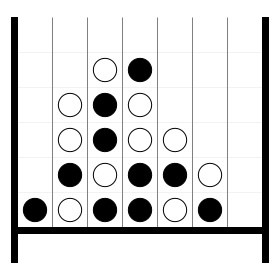
\includegraphics[width=0.2\textwidth]{intro2.png}
    \label{fig:intro}
\end{figure}
    \textbf{Connect Four} is a two-player game played on a vertical 7-column, 6-row grid where players take turns dropping colored discs into the slots, aiming to connect four discs of their color horizontally, vertically, or diagonally.
\end{frame}

%------------------------------------------------

\begin{frame}{\makebox[0.95\linewidth][l]{Properties \hfill \textcolor{lightgray}{\insertsection}}}
\begin{itemize}
    \item \textbf{Deterministic:} Outcome fully determined by player actions. $S_{t+1}, R_{t} = p(S_t, a_t)$
    \item \textbf{Episodic:} Sequence of actions leading to a terminal state. Episode: $\{(S_1, a_1), \dots, (S_T, a_T)\}$
    \item \textbf{Two-Player:} Players 1 and 2 alternate moves, strategies $\pi_1$ and $\pi_2$. % Corrected line
    \item \textbf{Zero-Sum:} Rewards sum to zero.  $R_1 = -R_2$. Terminal rewards: Win (+1/-1), Draw (0/0)
    \item \textbf{Perfect Information:} Both players have complete knowledge of the current state.
    \item \textbf{Solvability:} Solved. Player 1 can always win with optimal play (Wikipedia). No readily available solvers for testing.
\end{itemize}
\end{frame}

%------------------------------------------------

\begin{frame}{\makebox[0.95\linewidth][l]{Complexity \hfill \textcolor{lightgray}{\insertsection}}}
    \begin{itemize}
        \item \textbf{Trajectory Length:} Max 42 moves (7 columns x 6 rows).
        \item \textbf{State Space:}
            \begin{itemize}
                \item Naive: $3^{42} \approx 1.1 \times 10^{20}$
                \item Improved: $\approx 4.5 \times 10^{12}$ states
                \item Storage: $4.5 \times 10^{12} \text{ states} \times 8 \text{ bytes/state} = 36 \text{ TB}$ (64 bit state representation)
            \end{itemize}
        \item \textbf{Tabular Methods:} Infeasible due to large state space.
    \end{itemize}
\end{frame}

%------------------------------------------------
\section{Implementation}
%------------------------------------------------

\begin{frame}{\makebox[0.95\linewidth][l]{Framework \hfill \textcolor{lightgray}{\insertsection}}}

\textbf{Framework:} JAX provides a high-performance framework for computational efficiency and flexibility, allowing for scalable and efficient development of machine learning algorithm.

\vspace{2.5em}

\textbf{JAX Features:}
\begin{itemize}
    \item JIT Compilation
    \item GPU/TPU Acceleration
    \item Efficient Vectorization (vmap)
    \item Automatic Parallelization (pmap)
    \item Functional Programming (Pure Functions)
\end{itemize}
\end{frame}

%------------------------------------------------


\begin{frame}{\makebox[0.95\linewidth][l]{Libraries with links \hfill \textcolor{lightgray}{\insertsection}}}
\begin{itemize}
    \item \href{https://github.com/google-deepmind/mctx}{\texttt{mctx}}: JAX-native MCTS implementations.
    \item \href{https://github.com/sotetsuk/pgx}{\texttt{pgx}}: Game environment simulation, diverse games, fast parallelization.
    \item \href{https://github.com/google-deepmind/dm-haiku}{\texttt{Haiku}}: Neural network building and training in JAX.
    \item \href{https://github.com/deepmind/optax}{\texttt{optax}}: Gradient processing and optimization.
\end{itemize}
\end{frame}


%------------------------------------------------
\section{MCTS Review}
%------------------------------------------------


\begin{frame}{\makebox[0.95\linewidth][l]{Monte Carlo Tree Search (MCTS) \hfill \textcolor{lightgray}{\insertsection}}}
\vspace{1.5em}
Monte Carlo Tree Search is a decision-making algorithm that explores a decision space by constructing a search tree through repeated simulations. Given a computation budget it balances exploration and exploitation to refine the root node policy.

\vspace{2.5em}

\begin{figure}[h]
    \centering
    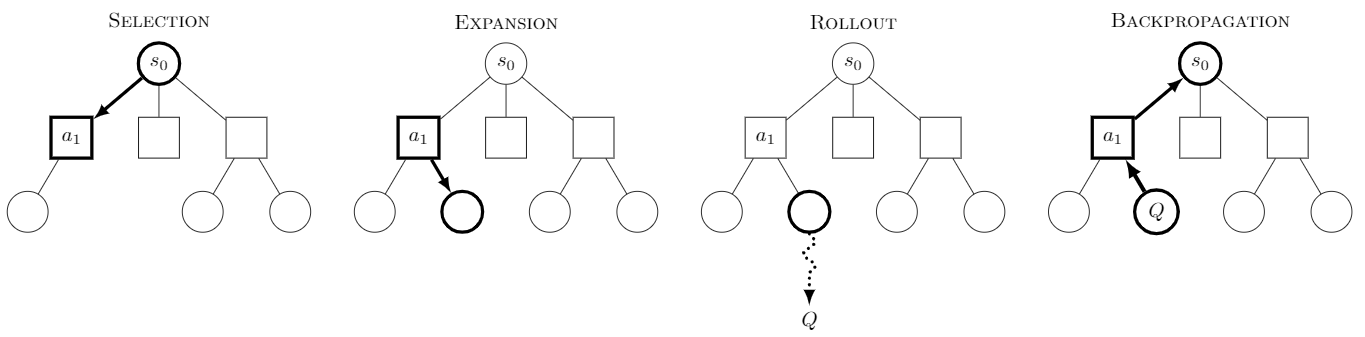
\includegraphics[width=1.0\textwidth]{mcts.png}
    \label{fig:intro}
\end{figure}
\end{frame}

%------------------------------------------------
%
%\begin{frame}{\makebox[0.95\linewidth][l]{Selection \hfill \textcolor{lightgray}{\insertsection}}}
%\vspace{1.5em}
%Traverses the tree from the root to a leaf node using a selection policy that balances exploration and exploitation, considering: visit counts $N$ , mean value $Q$, prior policy $P$ , reward $R$, and state transition $S$.
%\vspace{1.5em}
%\begin{figure}[h]
%    \centering
%    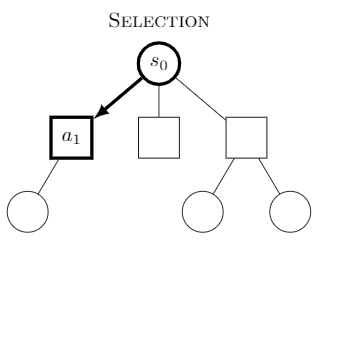
\includegraphics[width=0.4\textwidth]{selection.png}
%    \label{fig:intro}
%\end{figure}
%\end{frame}
%
%%------------------------------------------------
%
%\begin{frame}{\makebox[0.95\linewidth][l]{Expansion \hfill \textcolor{lightgray}{\insertsection}}}
%\vspace{1.5em}
%Adds a new child node to the selected leaf node, representing a possible action from that state
%\vspace{1.5em}
%\begin{figure}[h]
%    \centering
%    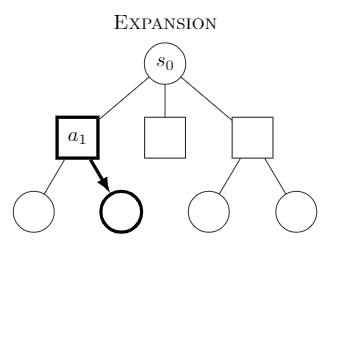
\includegraphics[width=0.4\textwidth]{expansion.png}
%    \label{fig:intro}
%\end{figure}
%\end{frame}
%
%%------------------------------------------------
%
%\begin{frame}{\makebox[0.95\linewidth][l]{Rollout or Simulation \hfill \textcolor{lightgray}{\insertsection}}}
%\vspace{1.5em}
%Approximate the value function of the leaf state, can be random rollout or neural network approximation
%\vspace{0.7em}
%\begin{figure}[h]
%    \centering
%    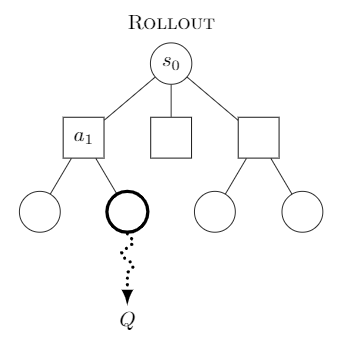
\includegraphics[width=0.4\textwidth]{approximation.png}
%    \label{fig:intro}
%\end{figure}
%\end{frame}
%
%%------------------------------------------------
%
%\begin{frame}{\makebox[0.95\linewidth][l]{Backpropagation \hfill \textcolor{lightgray}{\insertsection}}}
%\vspace{1.5em}
%Updates the statistics of the nodes visited during selection and expansion based on the simulation outcome.  These statistics (e.g., win counts, visit counts) inform the selection policy in subsequent iterations, gradually biasing the search towards promising actions
%\vspace{1.0em}
%\begin{figure}[h]
%    \centering
%    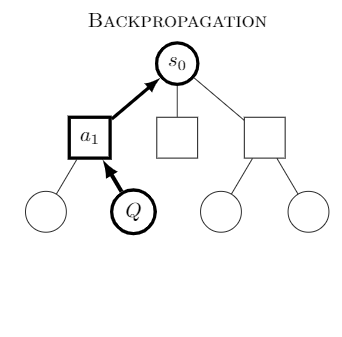
\includegraphics[width=0.4\textwidth]{backpropagation.png}
%    \label{fig:intro}
%\end{figure}
%\end{frame}
% 
%%------------------------------------------------

\begin{frame}{\makebox[0.95\linewidth][l]{MCTX Library API \hfill \textcolor{lightgray}{\insertsection}}}
To perform a MCTS search using the MCTX library, two main functions must be provided:

\medskip
\textbf{RootFnOutput(state):}
\begin{itemize}
    \item Specifies the representation of the root state.
    \item Returns the prior logits and the estimated value of the root state.
\end{itemize}

\medskip
\textbf{recurrent\_fn(state, action):}
\begin{itemize}
    \item Encapsulates the environment dynamics.
    \item Returns the reward, discount factor, and for the new state, the prior logits and value.
\end{itemize}


\vspace{3.0em}
    The search returns \textbf{action\_weight}, representing the updated root node policy (policy\_out).
\end{frame}

%------------------------------------------------
\section{Common implementation details}
%------------------------------------------------


\begin{frame}{\makebox[0.95\linewidth][l]{Negative Discount Factor \hfill \textcolor{lightgray}{\insertsection}}}

In alternating-turn games, a negative discount factor (\(\gamma = -1\)) is used to invert value estimates between players:

\medskip
\[
    V(S_t) = \mathbb{E} \left[ r_{t+1} + \gamma \cdot V(S_{t+1}) \right] = \mathbb{E} \left[ r_{t+1} + (-1) \cdot V(S_{t+1}) \right]
\]
\begin{itemize}
    \item \(S_t\): Current state (Player 1’s turn).
    \item \(S_{t+1}\): Next state (Player 2’s turn), where the value \(V(S_{t+1})\) represents the opponent's optimal value.
\end{itemize}

\medskip
This inversion maintains the zero-sum property by ensuring that a high value for one player corresponds to a low value for the opponent.
\end{frame}

%------------------------------------------------

\begin{frame}{\makebox[0.95\linewidth][l]{Neural Network \hfill \textcolor{lightgray}{\insertsection}}}
The neural network is a custom \textbf{ResNet}, a convolutional network with residual connections and batch normalization. It has two output heads:

\medskip
\[
l, v' = \text{ResNet}_\theta(S_t)
\]
\medskip
\textbf{1. Policy Head:} Produces a probability distribution over possible actions:
\[
\pi(a \mid S_t) \approx \hat{\pi}(a \mid S_t) = \text{softmax}(l)
\]

\textbf{2. Value Head:} Outputs a scalar value approximating the value function:
\[
V(S_t) \approx \hat{V}(S_t) = v'
\]

\end{frame}

%------------------------------------------------
\section{Naive MCTS}
%------------------------------------------------


\begin{frame}{\makebox[0.95\linewidth][l]{Description \hfill \textcolor{lightgray}{\insertsection}}}
    Naive implementation of Monte Carlo Tree Search:

    \medskip
    \begin{itemize}
    \item \textbf{no learning}
    \item MCTS
            \begin{itemize}
                \item policy: uniform
                \item value: single random rollout
            \end{itemize}
\end{itemize}

\end{frame}

%------------------------------------------------

\begin{frame}{\makebox[0.95\linewidth][l]{Pseudocode MCTS Inference\hfill \textcolor{lightgray}{\insertsection}}}
\begin{figure}[h]
    \centering
    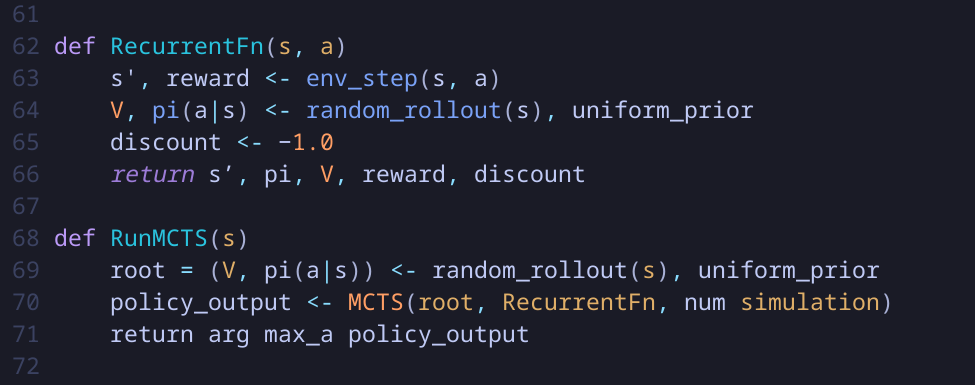
\includegraphics[width=0.9\textwidth]{naive_mcts_algo.png}
    \label{fig:intro}
\end{figure}
\end{frame}

%\begin{frame}{\makebox[0.95\linewidth][l]{Pseudocode Inference\hfill \textcolor{lightgray}{\insertsection}}}
%  \begin{algorithmic}
%    \Function{RecurrentFn}{s, a}
%      \State $s', reward \gets env.step(s, a)$
%      \State $(logit', value')\gets uniform\_prior, random\_rollout(s')$
%      \State $discount \gets -1.0 $
%      \State \textbf{return} s', logit', value', reward, discount
%    \EndFunction
%  \end{algorithmic}
%
%    \medskip
%    \medskip
%  \begin{algorithmic}
%    \Function{RunMCTS}{$s$}
%      \State $root = (logit, value)\gets uniform\_prior, random\_rollout(s)$
%
%
%      \State $policy\_output \gets MCTS(root, RecurrentFn, num\_simulation)$
%
%      \State $\textbf{return} \arg\max_a policy\_output$
%
%      \EndFunction
%  \end{algorithmic}
%\end{frame}

%------------------------------------------------

\begin{frame}{\makebox[0.95\linewidth][l]{Example Policy\_Out \hfill \textcolor{lightgray}{\insertsection}}}
    \begin{columns}[c] % The "c" option specifies centered vertical alignment while the "t" option is used for top vertical alignment
        \column{.45\textwidth} % Left column and width
\begin{figure}[h]
    \centering
    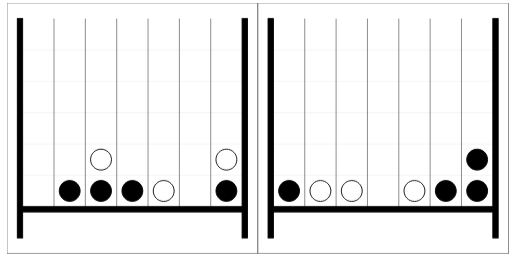
\includegraphics[width=0.9\textwidth]{state.png}
    \label{fig:intro}
    Value = [-1, -1]
\end{figure}
        \column{.45\textwidth} % Left column and width
\begin{figure}[h]
    Policy output
    \centering
    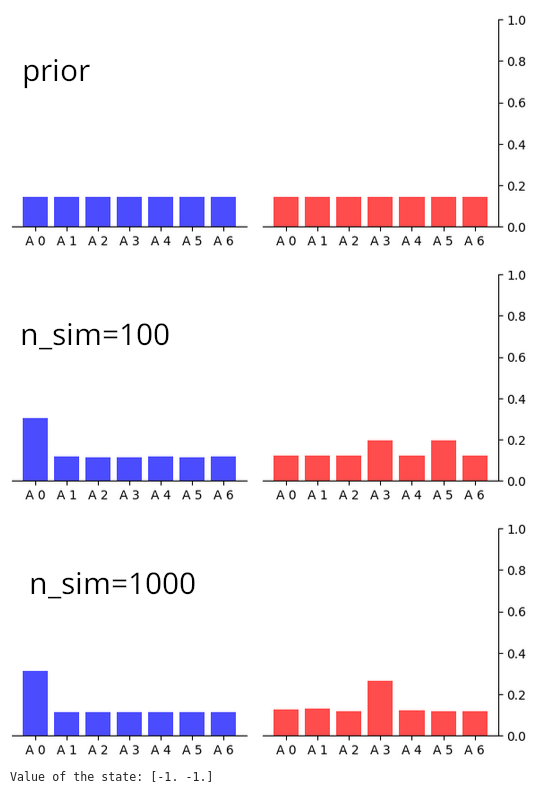
\includegraphics[width=0.7\textwidth]{prob2.png}
    \label{fig:intro}
\end{figure}
    \end{columns}
\end{frame}

%------------------------------------------------
\section{Reinforce Baseline}
%------------------------------------------------

\begin{frame}{\makebox[0.95\linewidth][l]{Description \hfill \textcolor{lightgray}{\insertsection}}}
    Reinforce baseline algorithm:

    \medskip
    \begin{itemize}
    \item Policy based algorithm
    \item no MCTS
    \item on policy, batch
    \item neural network function and policy approximation
\end{itemize}
\end{frame}

\begin{frame}{\makebox[0.95\linewidth][l]{Pseudocode \hfill \textcolor{lightgray}{\insertsection}}}
    \begin{textblock*}{\paperwidth}(0mm,20mm) % Position at (0,0)
        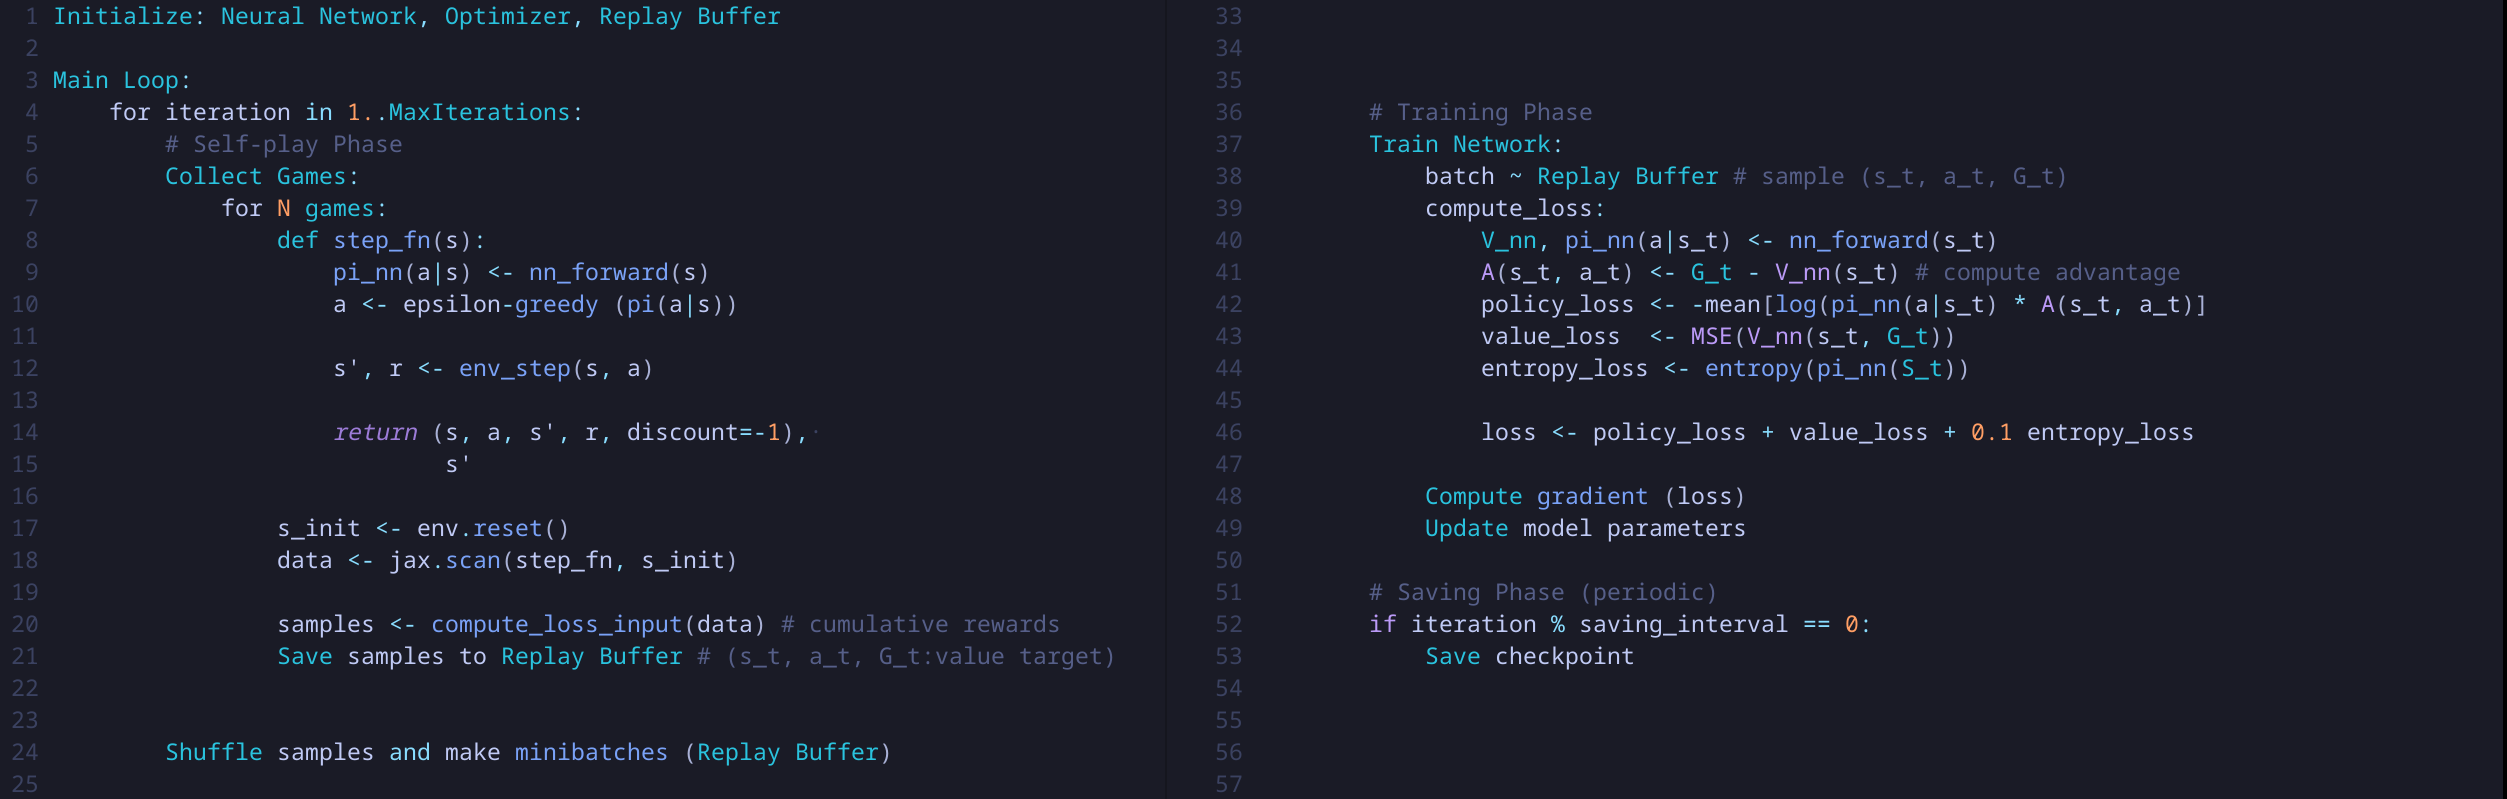
\includegraphics[width=\paperwidth,height=\paperheight,keepaspectratio]{reinforce_algo.png}
    \end{textblock*}
\end{frame}

%\begin{frame}{\makebox[0.95\linewidth][l]{Pseudocode\hfill \textcolor{lightgray}{\insertsection}}}
%    \begin{columns}[c] % The "c" option specifies centered vertical alignment while the "t" option is used for top vertical alignment
%        \column{.45\textwidth} % Left column and width
%    \scriptsize
%      \begin{algorithmic}
%          \State \textbf{Initialize: Neural Network, Optimizer, Replay Buffer}
%
%    \State \textbf{Main Loop:}
%    \For{iteration = 1 to MaxIterations}
%        \State \textbf{Self-play Phase}
%        \State \quad \textbf{Collect Games:}
%        \For{N games}
%            \State \quad $state \gets \text{env.reset()}$
%            \State \quad $game\_history \gets []$
%            \While{not terminated}
%                \State \quad \textbf{Run MCTS:}
%                \For{M simulations}
%                    \State \quad \text{Expand nodes using network predictions}
%                    \State \quad \text{Backpropagate values}
%                \EndFor
%                \State \quad \text{Get action probabilities from MCTS}
%                \State \quad \text{Store state and action probabilities}
%                \State \quad \text{Take action, observe reward}
%                \State \quad $state \gets \text{next state}$
%            \EndWhile
%            \State \quad \text{Compute value targets (discounted cumulative rewards)}
%            \State \quad \text{Save game to replay buffer}
%        \EndFor
%    \EndFor
%  \end{algorithmic}
%
%        \column{.45\textwidth} % Left column and width
%        aaa
%    \end{columns}
%\end{frame}

\begin{frame}{\makebox[0.95\linewidth][l]{Loss \hfill \textcolor{lightgray}{\insertsection}}}
    \textbf{Total Loss:}
    \[
    L = \mathcal{L}_{\text{policy}} + \mathcal{L}_{\text{value}} + 0.1 \times \mathcal{L}_{\text{entropy}}
    \]

    \vspace{0.3cm}
    \textbf{Where:}
    \[
    \mathcal{L}_{\text{policy}} = - \mathbb{E} \left[ \log \hat{\pi}(a_t \mid S_t) \cdot A(S_t, a_t)  \right]
    \]
    \[
    A(S_t, a_t) = G_t - \hat{V}(S_t)
    \]
    \[
    \mathcal{L}_{\text{value}} = \mathbb{E} \left[ \left( \hat{V}(S_t) - G_t \right)^2  \right]
    \]
    \[
    \mathcal{L}_{\text{entropy}} = - \mathbb{E} \left[ \sum_a \pi(a \mid S_t) \log \pi(a \mid S_t)  \right]
    \]

    \textbf{Gradient Clipping}: ensures that the gradients do not exceed a specified threshold, preventing exploding gradients.
\end{frame}


\begin{frame}{\makebox[0.95\linewidth][l]{Loss plot \hfill \textcolor{lightgray}{\insertsection}}}
\begin{figure}[h]
    \centering
    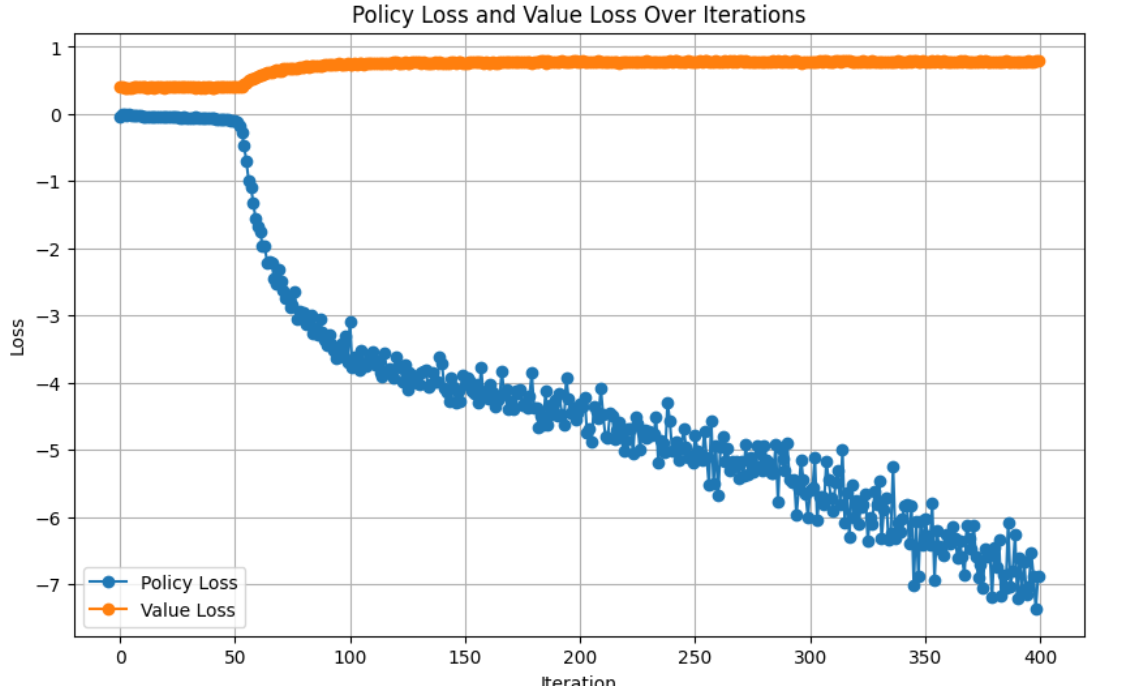
\includegraphics[width=0.9\textwidth]{reinforce_loss.png}
    \label{fig:intro}
\end{figure}
\end{frame}

\begin{frame}{\makebox[0.95\linewidth][l]{Loss \hfill \textcolor{lightgray}{\insertsection}}}
    Even with loss improvements, divergence still occurs.

    \vspace{0.5cm}
    \textbf{The Deadly Triad:}\\
    \vspace{0.5cm}
    \begin{tabular}{@{}l@{\hspace{1cm}}l@{}}
        \qquad Bootstrapping            & \textcolor{red}{\texttimes} \\[5pt]
        \qquad Function Approximation   & \textcolor{green}{\checkmark} \\[5pt]
        \qquad Off-Policy     & \textcolor{red}{\texttimes}
    \end{tabular}
\end{frame}


%------------------------------------------------
\section{Alphazero}
%------------------------------------------------

\begin{frame}{\makebox[0.95\linewidth][l]{Description \hfill \textcolor{lightgray}{\insertsection}}}
    Alphazero algorithm

    \medskip
    \begin{itemize}
    \item MCTS
            \begin{itemize}
                \item policy: neural network policy head
                \item value: neural network value head
            \end{itemize}
\end{itemize}
\end{frame}

\begin{frame}{\makebox[0.95\linewidth][l]{Pseudocode \hfill \textcolor{lightgray}{\insertsection}}}
    \begin{textblock*}{\paperwidth}(0mm,18mm) % Position at (0,0)
        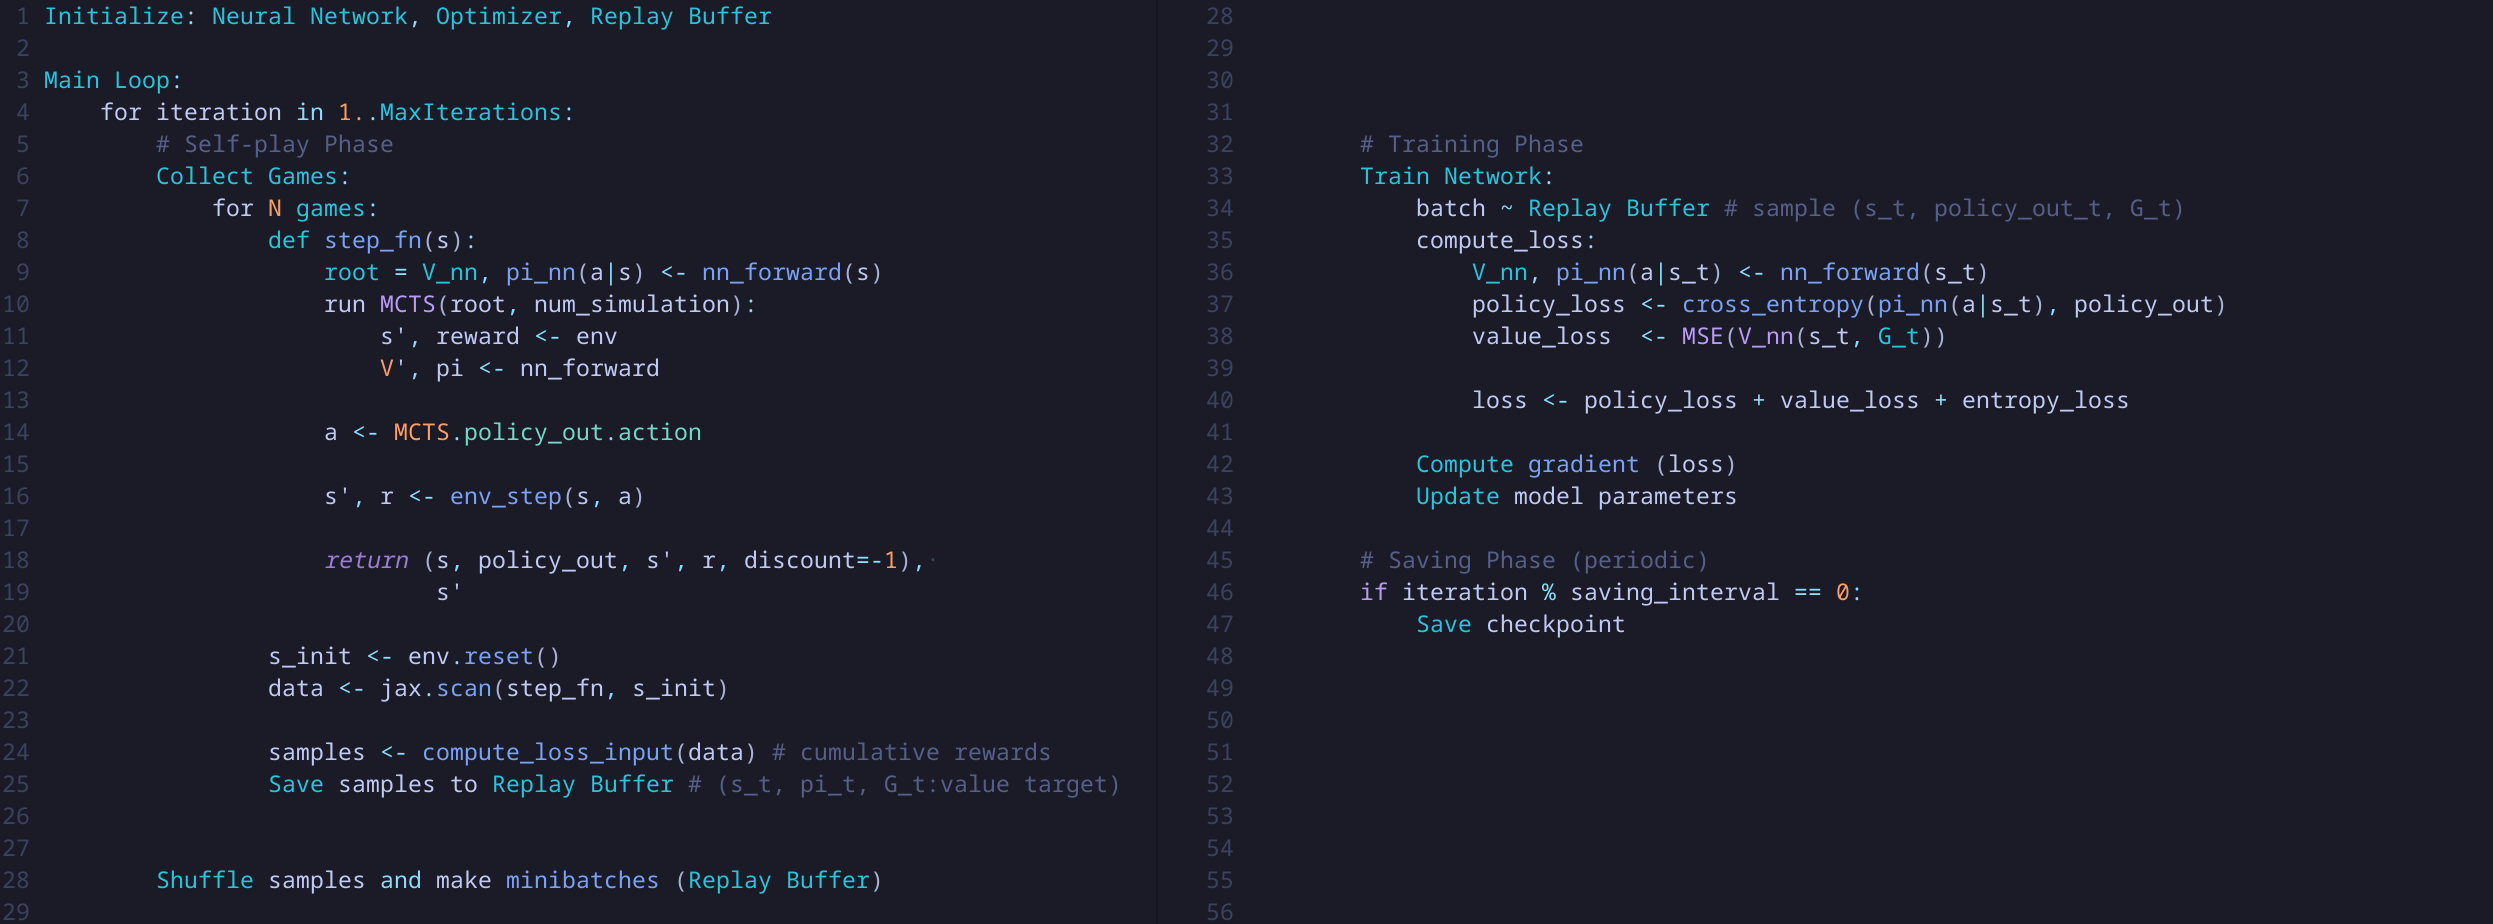
\includegraphics[width=\paperwidth,height=\paperheight,keepaspectratio]{alphazero_algo.png}
    \end{textblock*}
\end{frame}

\begin{frame}{\makebox[0.95\linewidth][l]{Loss \hfill \textcolor{lightgray}{\insertsection}}}
    \textbf{Total Loss:}
    \[
    L = \mathcal{L}_{\text{policy}} + \mathcal{L}_{\text{value}} 
    \]

    \vspace{0.3cm}
    \textbf{Where:}
    \[
        \mathcal{L}_{\text{policy}} = - \mathbb{E}_{a \sim policy\_out} \left[ \log \hat{\pi}(a)  \right]
    \]
    \[
    \mathcal{L}_{\text{value}} = \mathbb{E} \left[ \left( \hat{V}(S_t) - G_t \right)^2  \right]
    \]

\end{frame}

\begin{frame}{\makebox[0.95\linewidth][l]{Loss plot \hfill \textcolor{lightgray}{\insertsection}}}
\begin{figure}[h]
    \centering
    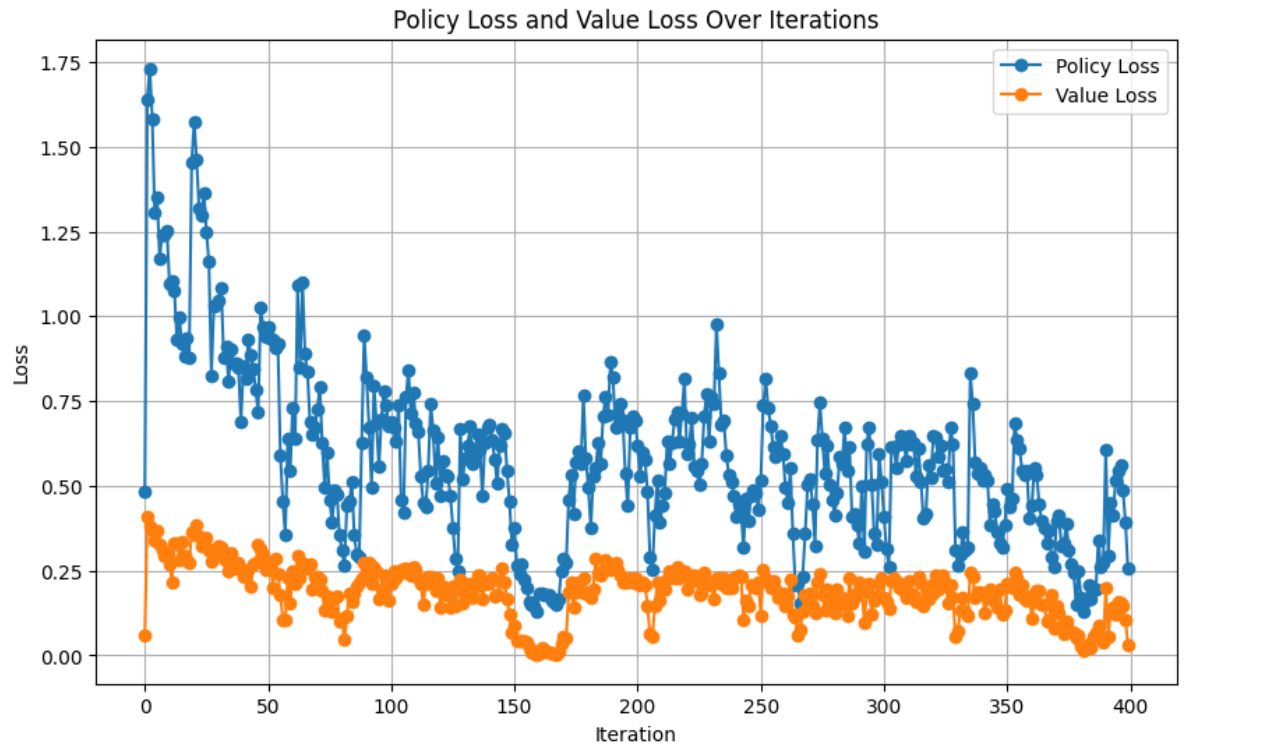
\includegraphics[width=0.9\textwidth]{alphazero_loss_plot1.png}
    \label{fig:intro}
\end{figure}
\end{frame}

\begin{frame}{\makebox[0.95\linewidth][l]{Loss plot 2 \hfill \textcolor{lightgray}{\insertsection}}}
With better training: increase num. MCTS simulation, batch size, neural network
\begin{figure}[h]
    \centering
    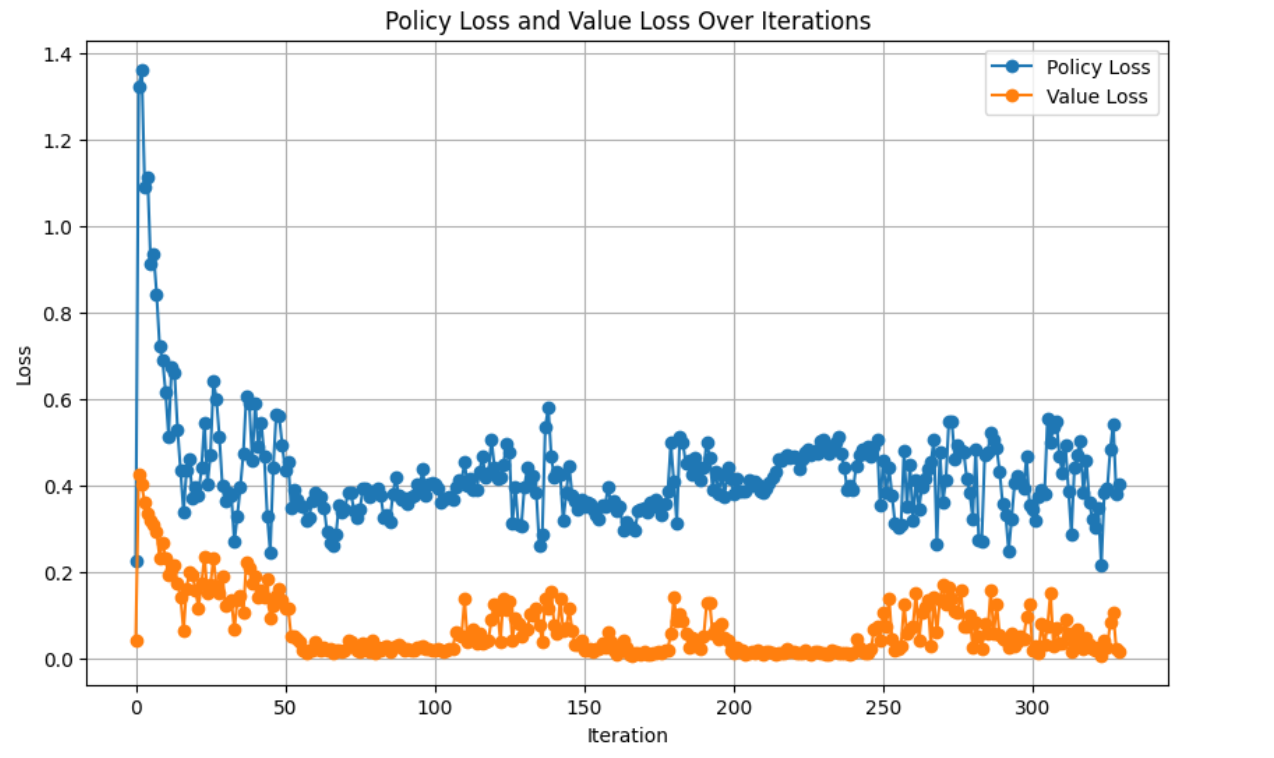
\includegraphics[width=0.8\textwidth]{alphazero_loss_plot2.png}
    \label{fig:intro}
\end{figure}
\end{frame}

\begin{frame}{\makebox[0.95\linewidth][l]{Inference MCTS vs One-shot\hfill \textcolor{lightgray}{\insertsection}}}
\begin{figure}[h]
    \centering
    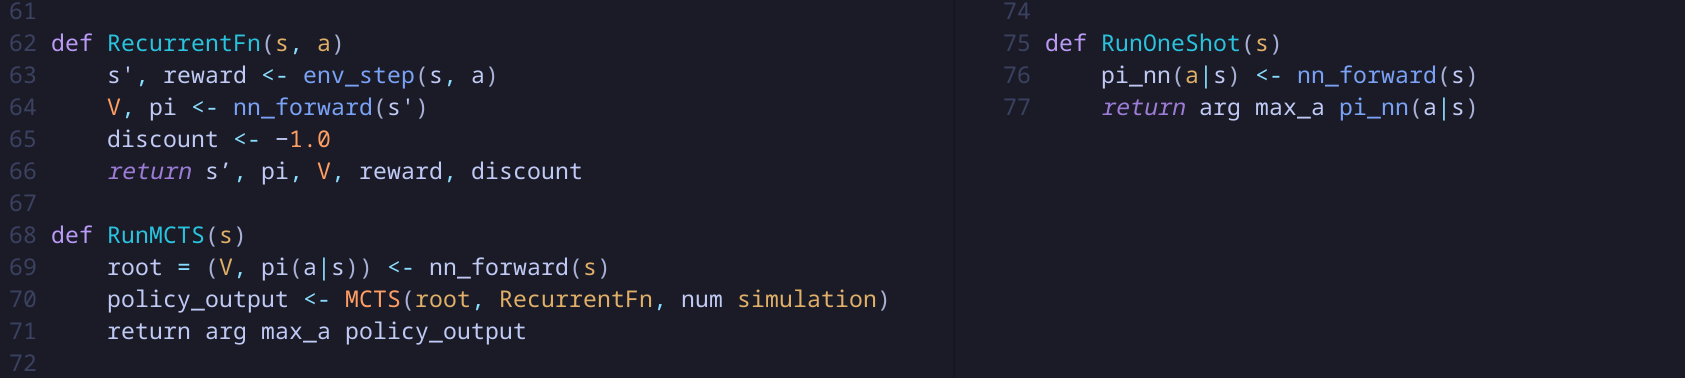
\includegraphics[width=1\textwidth]{inference.png}
    \label{fig:intro}
\end{figure}
\end{frame}

\begin{frame}{\makebox[0.95\linewidth][l]{Example Network forward\hfill \textcolor{lightgray}{\insertsection}}}
\begin{figure}[h]
    \centering
    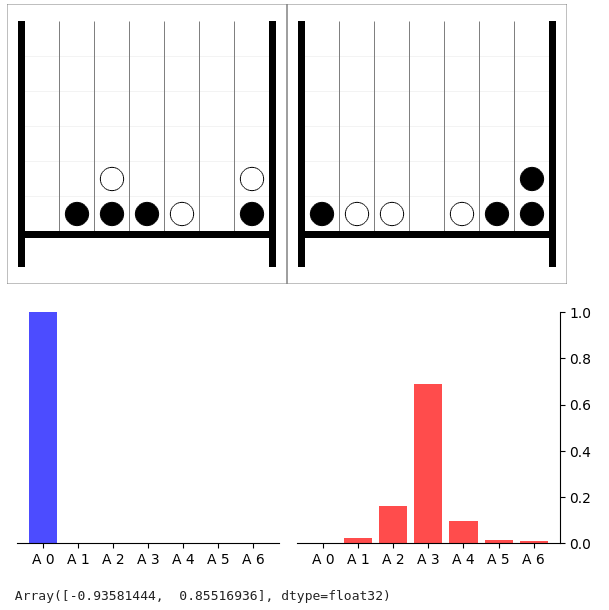
\includegraphics[width=0.5\textwidth]{network_forward.png}
    \label{fig:intro}
\end{figure}
\end{frame}


%------------------------------------------------
\section{Conclusion}
%------------------------------------------------
\begin{frame}{\makebox[0.95\linewidth][l]{Evaluation \hfill \textcolor{lightgray}{\insertsection}}}
    \Huge{\centerline{\textbf{Notebook games and live play}}}
\end{frame}

\begin{frame}{\makebox[0.95\linewidth][l]{Future Experiments \hfill \textcolor{lightgray}{\insertsection}}}
    \begin{itemize}
    \item hyper-parameter tuning for better training
    \item longer training
    \item network architecture
            \begin{itemize}
                \item increase capacity
                \item transformer architecture
            \end{itemize}

    \item MCTS: test different selection algorithm
\end{itemize}
\end{frame}

\begin{frame}{References}
    \footnotesize
    \nocite{*}
    \bibliography{reference.bib}
    \bibliographystyle{apalike}
\end{frame}

%------------------------------------------------

\begin{frame}
    \Huge{\centerline{\textbf{Thank you for your attention!  }}}
\end{frame}

%----------------------------------------------------------------------------------------

\end{document}
